This chapter presents the results we collected after performing the user study on Fat Finger interaction technique. We decided to focus on 5 basic categories, which include the most significant information we collected and analysed. We present the results for Task Completion Time, Offsets, Learning Curve, Re-Entries - Re-Touches and Subjective Preferences. We also refer to the categories of the trials with the shortages presented in Table \ref{tab:typeIDnames}. This will help the reader to better understand and interpret the various graphs presented onwards.

\begin{table}[H]
\centering
\begin{tabular}{l | c | c }
\textbf{Name} & \textbf{Code-Name} & \textbf{TypeID} \\
\hline
\hline
Feedback \& Discrete & FD & 1 \\
\hline
Feedback \& Continuous & FC & 2 \\
\hline
No Feedback \& Discrete & NFD & 3 \\
\hline
No Feedback \& Continuous & NFC & 4 \\
\end{tabular}
\caption{Code names for the 4 categories of trials}
\label{tab:typeIDnames}
\end{table}


%%%%%%%%%%%%%%%%%%%%%%%%%%%%%
%%%%%%%%%%%%%%%%%%%%%%%%%%%%%
%%%%%%%%%%%%%%%%%%%%%%%%%%%%%
%%%%%%%%%%%%%%%%%%%%%%%%%%%%%
%%%%%%%%%%%%%%%%%%%%%%%%%%%%%
%%%%%%%%%%%%%%%%%%%%%%%%%%%%%
\section{Task Completion Time}
\label{sec:resultsTaskCompletionTime}

Task completion time is a parameter that counts the total time the participant spent on a specific trial. As mentioned in section \ref{sec:monitoring}, the timer fires when the first touch is performed and stops counting when the confirming sound is being played, which indicates that we successfully hit the target. Also in Feedback trials we use the Dwell selection technique which, requires a user to stay inside the target for 1 second. In No-Feedback trials there is no such time constraint, since we use the QuickRelease method (no obligatory delay) to perform target selection. 

We performed a $4 * 7$ (TypeID $*$ N) within subjects ANalysis Of VAriance (ANOVA) \cite{anova}, using the aggregated values of total time. We use ANOVA to determine if the mean values for offset are statistically different. Of course, we can export basic information about the means by just comparing them, but we want to know what do these directional differences in the means infer about our results. ANOVA is able to determine if the differences between condition means are significant.

\begin{figure}[H]
\centering
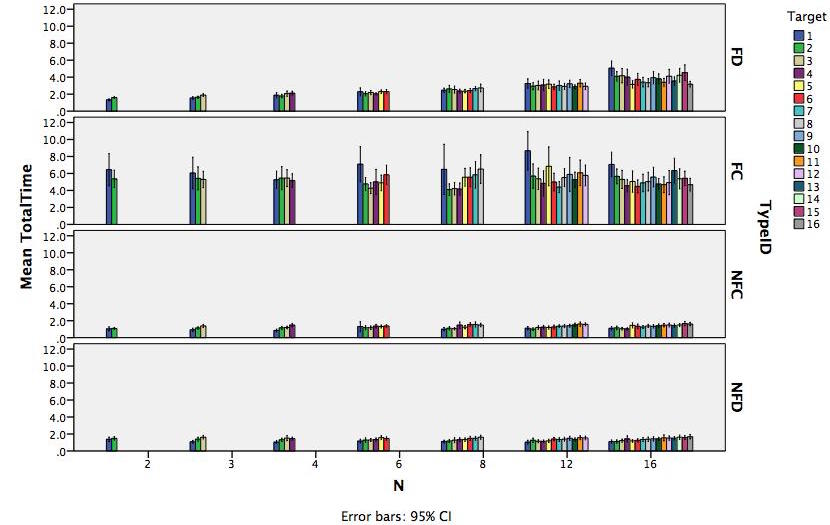
\includegraphics[width=\textwidth]{figures/meanTotalTime}
\caption{Total Time panelled by TypeID  - 95\% Confidence Interval}
\label{fig:meanTotalTime}
\end{figure}

Figure \ref{fig:meanTotalTime} illustrates the aggregated task completion time values, panel-by typeID and cluster-by the number of buckets (N).
 We found that Mauchly's Test of Sphericity is violated for all Type of Trial (TypeID), number of elements (N), and also their combination (TypeID*N). That means that the type of the trial, the number of elements and their combination have a significant effect on completion time. We found that Grand Mean is \emph{2.619} seconds (STD = \emph{0.142s}). Feedback \& Discrete (M = \emph{2.387s} STD = \emph{0.084s}) was really fast, taking into consideration that it expects \emph{1s} delay to confirm target selection.
  No Feedback \& Discrete (M = \emph{1.237s} and STD = \emph{0.093s}) and No Feedback \& Continuous (M = \emph{1.365s} and STD = \emph{0.013s}) were ranked almost equally and were the fastest. Feedback \& Continuous (\emph{M = 5.485} and \emph{STD = 0.457}) was the slowest one, but this can be partly explained from the fact that on the one hand, it contained the smallest targets, and on the other, the user had to pass the \emph{1s} inside target delay. Stay for \emph{1s} inside a designated small area can be really difficult under certain conditions.

Table \ref{tab:totaTimeAnova} presents the mean differences between all possible combination of the type of Trials (TypeID). As we can see, and  as already stated, Mean differences are really significant for all possible combinations.

\begin{table}[H]
\centering
\begin{tabular}{c | c | c | c}
TypeID (i) & TypeID (j) & Mean Difference (i-j) & Sig. \\
\hline \hline
FD      &   FC      &   -3.098      & 0.000 \\
FD      &   NFD     &   1.151       & 0.000 \\
FD      &   NFC     &   1.022       & 0.000 \\
FC      &   NFD     &   4.249       & 0.000 \\
FC      &   NFC     &   4.120       & 0.000 \\
NFD     &   NFC     &   -0.129      & 0.002
\end{tabular}
\caption{Task Completion Time: Mean differences among the different types of Trials}
\label{tab:totaTimeAnova}
\end{table}

Type of Elements (N), is a parameter that specifies the size of the target for Discrete trials and also the position of it, depending on which is the target bucket out of the N specified. In Continuous trials the size of each trial is independent of the number of elements (N), and is stable. However, N limits the position of the target under a specific region. 
Lower values for N result in a wider space range (\emph{N=2} and \emph{TargetBucket=1} means that the target can be anywhere inside the lower semicircle), while higher values significantly narrow this range (\emph{N=16} and \emph{TargetBucket=1} means that the target will be somewhere really close to the minimum value).

We found that task completion time does not statistically differ for \emph{N = 2, 3, 4, 6, 8}. For all those different type of elements the Mean differences are not statistically different, thus we can conclude that they behave quite similarly. However, as expected, the scenario is different for 12 and 16 Elements. For \emph{N=12} we detect significant differences with \emph{N=2} (Sig. = 0.024) and \emph{N=3} (Sig. = 0.017), while for the rest we have no significant differences (Sig. values $>$ 0.05). However \emph{N=16} differs significantly with all the aforementioned \emph{N}'s, apart from \emph{N=12}. 

The combination of the number of Elements (N) and the type of Trials, in turn points out some other important results too. For FC, NFD and NFC we observe that the number of Elements does not influence that task completion time. We have very similar completion times which are independent of N. Specifically, for \emph{Feedback \& Continuous} time for all possible N's is around 5.485 seconds, for \emph{No Feedback \& Discrete} around 1.237 seconds and for \emph{No Feedback \& Continuous} around 1.365.
 However, interest is really triggered when we check the values for \emph{Feedback \& Discrete} targeting. The completion time  is significantly increased as the number of Elements increases. We start with \emph{1.460 s} for \emph{N=2} and we end up with \emph{3.858 s} for \emph{N=16}. Completion time accordingly gradually increases for all intermediate N values, which supports H5. For \emph{N=16} we have that bucket size is still bigger that the size of a continuous target (offset range including). We expect that for even smaller targets, as in \emph{Feedback \& Continuous}, the completion time will be even higher, as the target range is smaller. This claim indeed holds. We saw above that for FC the completion time is stable and independent on the number of elements (\emph{N}), which makes sense because in FC target size does not even change. Summarizing we can conclude that:
\emph{
\begin{itemize}
    \item When feedback is provided, completion time is highly dependent on the size of the target, increasing as the target size decreases. 
    \item When feedback is provided, completion time is statistically independent for N values up to 8 buckets.
    \item In No Feedback trials, completion time is independent of the size of the buckets.
\end{itemize}
}











%%%%%%%%%%%%%%%%%%%%%%%%%%%%%
%%%%%%%%%%%%%%%%%%%%%%%%%%%%%
%%%%%%%%%%%%%%%%%%%%%%%%%%%%%
%%%%%%%%%%%%%%%%%%%%%%%%%%%%%
%%%%%%%%%%%%%%%%%%%%%%%%%%%%%
%%%%%%%%%%%%%%%%%%%%%%%%%%%%%
\section{Offsets}
\label{sec:resultsOffset}

Offset is a parameter that generally represents the error for each trial. Error is measured by the percentage we were off the target. For instance, imagine that we have a target of type Continuous, placed on $x$ degrees, but we confirm selection at $y$ degrees, with $x\neq y$. Then the error is the difference of x and y, $x-y$. In other words it is the distance from the point we selected to the center of the target, compared to the whole range (\emph{360 degrees}). 
This difference produces a positive number if the confirmed contact size is bigger that the target's ($y>x$), and negative otherwise ($y<x$). Thus error rates can either be negative or positive depending on whether we performed selection before or after the target respectively. 
We also decided not to measure offset for FD trials, as there is no way that users can perform errors in those trials. Users were instructed to hit the target at whichever point inside its range, and not implicitly at the center of it. 
However, in No-Feedback trials the participant can confirm selection even if he is outside the target. Thus, error measurement is a much significant parameter, we need to analyse and export for those trials.

We aggregated the Offset values for each user, and with the aggregated offsets we performed a $3 * 7$ (\emph{TypeID $*$ N}) within subjects ANalysis Of VAriance. We found that Grand Offset Mean is \emph{11\%} , which can be translated into $39.6$ degrees ( \emph{11\% * 360 degrees}).
It is vital to mention that grand mean is much influenced from No Feedback trial values since, Feedback \& Continuous does not allow high values for error; simply because you can not select a target if you are outside the yellow lines. 
The range of the yellow lines is \emph{4\%}, thus errors are limited in the \emph{+-2\%} region. 
For Feedback \& Continuous trials, Mean offset is \emph{1,1\%} and STandard Deviation (STD) \emph{0,1\%}.
On the other hand, offset values are significantly increased in No Feedback trials. Well interestingly, both Feedback \& Discrete and No-Feedback \& Continuous share the same Mean offset values: \emph{Mean offset = 16,1\% and STD=1,1\%}.


Applying ANOVA and Post Hoc multiple means comparisons we found that \textbf{none} of the number of buckets (\emph{N}), the type of the Trials and the combination of them have an effect on the error rate - offset. Moreover we discovered that (including all possible N values) there is no significant difference between NFD and NFC (\emph{Sig = 1}).
We can conclude that the differences between those offset Means are likely due to chance and probably not due to the type of the trials.
Actually it is very interesting that NFD and NFC behave exactly the same along the experiment, which might infer that success rate of no feedback supported trials is not dependent on the size of the target.
Also, as expected FC behave differently ($Sig=0.000 \leq 0.05$) with both NFD and NFC.

Figure \ref{fig:meanOffset} illustrates the aggregated Offset values, panel-by typeID and cluster-by the number of buckets (\emph{N}). Observing the graph we can extract some meaningful results:

\begin{enumerate}
    \item \textbf{In FC error rates are always very small apart from a sudden increase they have for the last bucket of each N}. We attribute that to the fact that when the target was close to the maximum point (\emph{360 degrees}) users used to apply full pressure, ans so reach the maximum level, than trying to achieve high precision on the target by hitting it accurately. 

    \item \textbf{In NFD and NFC error rates follow a common pattern}. For the first buckets of each N they are positive, and they start going gradually negative as we move to the last buckets. This can be partly explained from the fact that average contact sizes are much easier to get achieved. When our finger simply touches the screen with, it is more likely to be somewhere between the minimum and the maximum area, that close to the limits. This is the natural position of our finger when are simply touching the screen.

    We realize then, that participants tend to go closer to this normalized area. They seem to have better control there, and more comfort too. This is probably why we observe that pattern on the graphs. When target are really close to the limits we tend to select areas that are closer to the normalized region than the correct ones.
\end{enumerate}
%%
%% FIG: Offset aggregated 
%%
\begin{figure}[H]
\centering
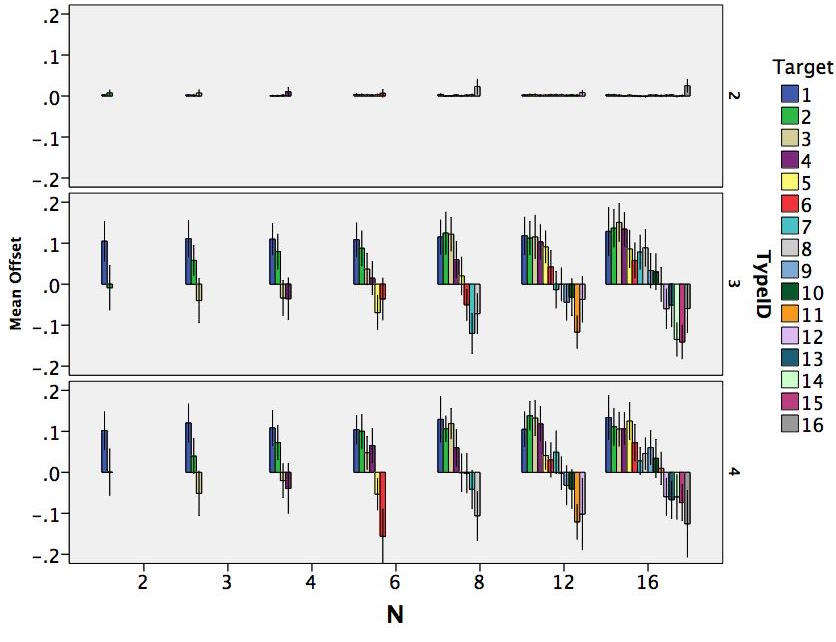
\includegraphics[width=\textwidth]{figures/meanOffset}
\caption{Offset aggregated - 95\% Confidence Interval}
\label{fig:meanOffset}
\end{figure}


After observing the error rates, it would be also nice to  take a look on the No Feedback trials success rate. Table \ref{tab:ffHitInside} presents the percentage of successful selections for both No Feedback \& Discrete and No Feedback \& Continuous. For Discrete targets the successful trials (\emph{33\%}) are much more than for the Continuous targets (\emph{11\%}).However they share the same error rates as mentioned above. How is that even possible?

Well, for Discrete targets we count the offset from the middle of each target. For instance,  if $N=2$ then the middle of the first bucket (down semicircle) is at \emph{90 degrees}. Even if the offset is \emph{25\%} ($=90 degrees$) then we are still inside the target, at the edge of it though. The same applies for higher \emph{N} values, but the 'permited'  offset is then narrower. Summarizing:

\emph{Offset values for Discrete targeting are not always considered as errors, as we measure offset from the center of the targets range. The real error can be calculated by the type:}   $RealErrorDisrete = OffsetValue - (TargetRange*0.5)$



\begin{table}[H]
\centering
\begin{tabular}{l || c | c }
 & Successful & Unsuccessful \\
\hline
\hline
NFD & 33.76\% & 66.16\% \\
NFC & 11.25\% & 88.75\% 
\end{tabular}
\caption{No Feedback: Percentage of successful hits}
\label{tab:ffHitInside}
\end{table}


% %%
% %% FIG: Hit Inside
% %%
% \begin{figure}[H]
% \centering
% \begin{subfigure}[b]{0.4\textwidth}
%     \centering
%     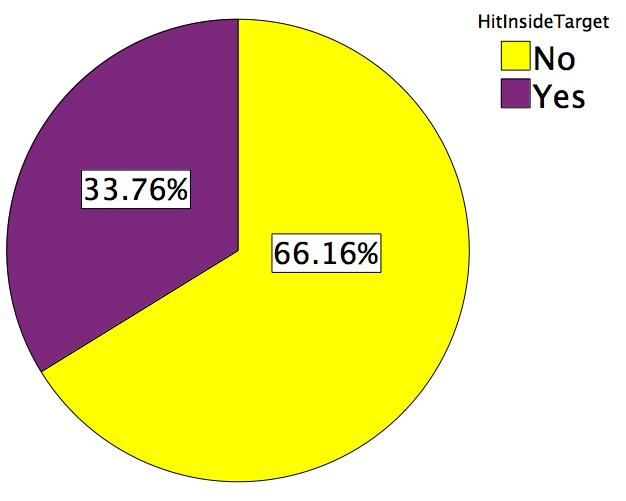
\includegraphics[width=\textwidth]{figures/hitInsideNFD}
%     \caption{Success ratio for No Feedback \& Discrete}
%     \label{fig:ffHitInsideNFD}
% \end{subfigure}
% \hfill
% \begin{subfigure}[b]{0.4\textwidth}
%     \centering
%     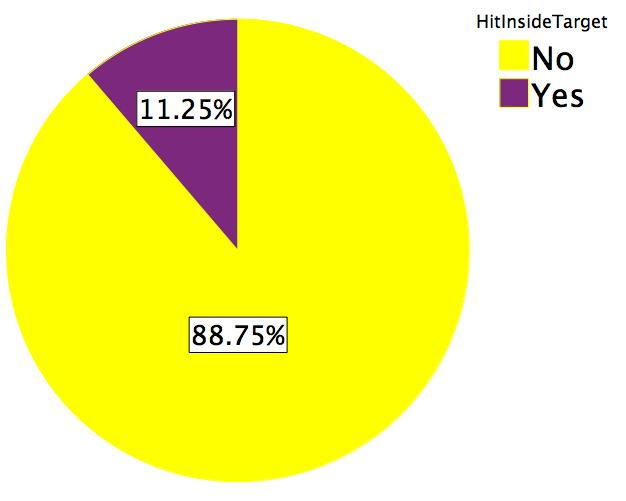
\includegraphics[width=\textwidth]{figures/hitInsideNFND}
%     \caption{Success ratio for No Feedback \& Continuous}
%     \label{fig:ffHitInsideNFND}
% \end{subfigure}
% \caption{Percentage of successfully hit No Feedback trials}
% \label{fig:ffHitInside}
% \end{figure}




%%%%%%%%%%%%%%%%%%%%%%%%%%%%%
%%%%%%%%%%%%%%%%%%%%%%%%%%%%%
%%%%%%%%%%%%%%%%%%%%%%%%%%%%%
%%%%%%%%%%%%%%%%%%%%%%%%%%%%%
%%%%%%%%%%%%%%%%%%%%%%%%%%%%%
%%%%%%%%%%%%%%%%%%%%%%%%%%%%%
\section{Learning Curve}
\label{resultsLearningCurve}

In section \ref{sec:FinalSequenceofTrials} we mentioned that training phase is not isolated from the rest of the experiment. Our approach is to use to use a 3-repetition design (Figure \ref{fig:ffRepetitions}), in which the first repetition will also act as the Learning phase, while the remaining 2 would just be the normal experiment. 
This way we are not eliminating learning from performing phase and most importantly, this give us the possibility to monitor the way and the pace the participants are getting used to this new interaction technique and observe the improvements of performance over time. In other words, this design provide us the appropriate tools for building the Learning Curve of Fat Finger.

    %%%%%%%%
    %%%%%%%%
    %%%%%%%%
\subsection{Total Time}
\label{sec:LCtotalTime}
We hypothesized (H3) that the average total time needed for the completion of each trial will be decreased over time. In other words we hypothesized that:

 $AverageTimeRepetition1 > AverageTimeRepetition2 > AverageTimeRepetition3$ 

Figure \ref{fig:learningCurveTotal} presents the average completion time learning curve in each repetition. We can observe that for repetition \emph{No 1} the mean time is just above \emph{3 seconds}. In Repetitions \emph{No 2} and \emph{No 3} the time decreased down to around \emph{2.5 seconds}. Thus we have a learning factor over time, especially between repetition \emph{No 1} and repetition \emph{No 2}. Repetition \emph{3} whilst not obviously improving the average trial time, is still contributing in the Learning effect in regards of specific trials; as I will thoroughly explain onwards. 
%%%%
%%%%
%% Total time Learinng Curve
%%%%
%%%%

\begin{figure}[H]
\centering
\begin{subfigure}[b]{0.45\textwidth}
    \centering
    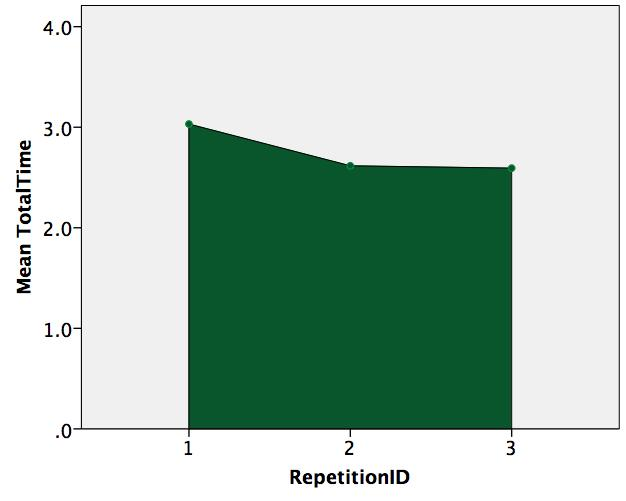
\includegraphics[width=\textwidth]{figures/learningCurveTotal}
    \caption{Learning Curve - Overall Total Time }
    \label{fig:learningCurveTotal}
\end{subfigure}
\hfill
\begin{subfigure}[b]{0.45\textwidth}
    \centering
    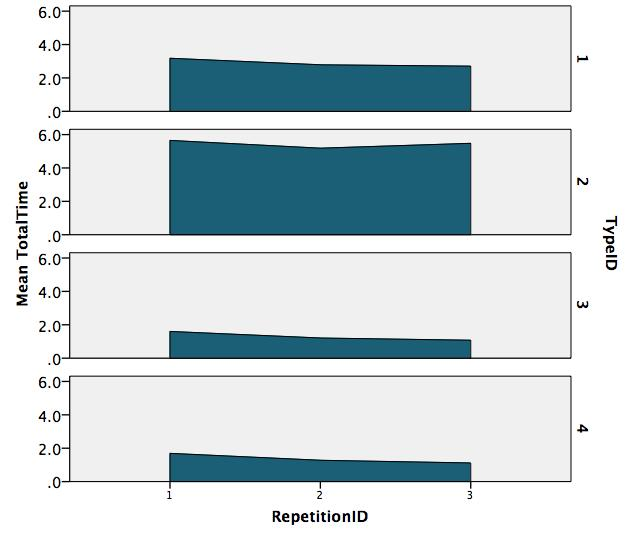
\includegraphics[width=\textwidth]{figures/learningCurve}
    \caption{Learning Curve - Time by TypeID}
    \label{fig:learningCurve}
\end{subfigure}
\caption{ Learning Curve - Task Completion Time}
\label{fig:learningCurveTotalTime}
\end{figure}



Figure \ref{fig:learningCurve} presents the average completion time learning curve in each repetition, panelled by Trial category (\emph{typeID}).
Learning curve for NFD ($TypeID = 3$) and NFC ($TypeID = 4$) depicts a continuous improvement of the average completion time among repetitions. However, the error rates learning curve as we point out in section \ref{sec:LCOffset}, have a completely reversed behaviour over time. 
Feedback \& Discrete learning curve follows the same behaviour as the overall time learning curve in \ref{fig:learningCurveTotal}.
On the other hand, Feedback \& continuous is the only type of trials for which, we do not observe continuous improvement over time. However, whilst being slower his error rates constantly decrease over time (section \ref{sec:LCOffset}). Thus, higher time values does not necessarily mean that our performance is being degraded.
 % Learning factor is a multi factor parameter, which mainly consists of the time and the error rate parameters. 

Taking into account the aforementioned graphs, we realize that there exist obvious learning improvements over time. However while for repetition \emph{No 1} to repetition \emph{No 2} we do observe significant learning factors, this is not that obvious for repetition \emph{No 3}. Mental and physical fatigue might have a share in this behaviour. While we do not have any measurement for fatigue to validate this claim, we can however extract some meaningful results from the assessments participants provided us at the end of each experiment. A short conclusion would be: if it was not for fatigue (mental and physical), learning curve might have been further decreased on repetition 3. 

%Finally, we encountered very few users that were really crummy during repetition 3, resulting in exponential increase in their total time. Ruling out these cases, we indeed have that average total time was further decreased on repetition 3. 

    %%%%%%%%
    %%%%%%%%
    %%%%%%%%
\subsection{Offset}
\label{sec:LCOffset}
In Figure \ref{fig:learningCurveOffset} we can observe the behaviour of Error rates along the repetitions, and use that knowledge to extract results regarding the error rates learning curve for all Feedback \& Continuous (blue), No Feedback \& Discrete (green) and No Feedback \& Continuous (red) trials. 

As we can notice, there is no significant improvement of the error rates over time, neither for FC (1,1\% - 1,1\% - 1\%), nor for NFC (16,3\% - 15,9\% - 16\%). The differences are on the 0,1\% scale which is not even noticeable. However in No Feedback \& Discrete trials (green) we do observe a drop of 2\% on the second repetition, but a slight increase (0,5\%) on the third one.
According to the aforementioned values, we realize that error rates are not subject to the same learning factor we experienced for Task Completion time in section \ref{sec:LCtotalTime}. However, the fact that we did not meet increasing values along the repetitions, is very promising. It infers that users are capable to maintain the same error rates, which are relatively low, along by decreasing their competition time.




%%%%
%%%%
%% OFFSET Learning Curve
%%%%
%%%%
% \begin{figure}[H]
% \centering
% \begin{subfigure}[b]{0.45\textwidth}
%     \centering
%     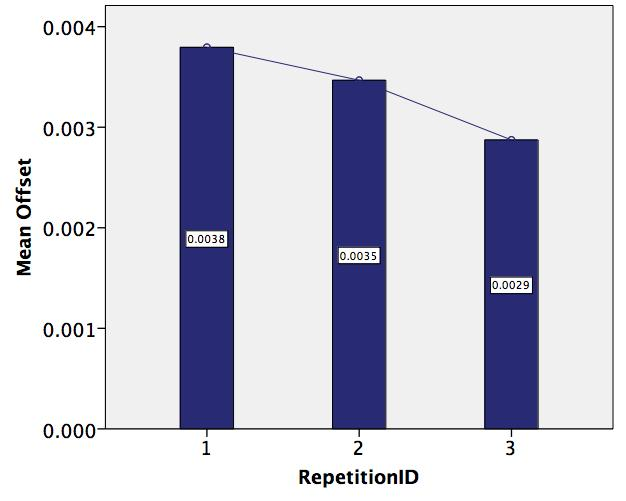
\includegraphics[width=\textwidth]{figures/learningCurveOffsetFC}
%     \caption{Error Rate Learning Curve - Feedback \& Continuous}
%     \label{fig:learningCurveOffsetFC}
% \end{subfigure}
% \hfill
% \begin{subfigure}[b]{0.45\textwidth}
%     \centering
%     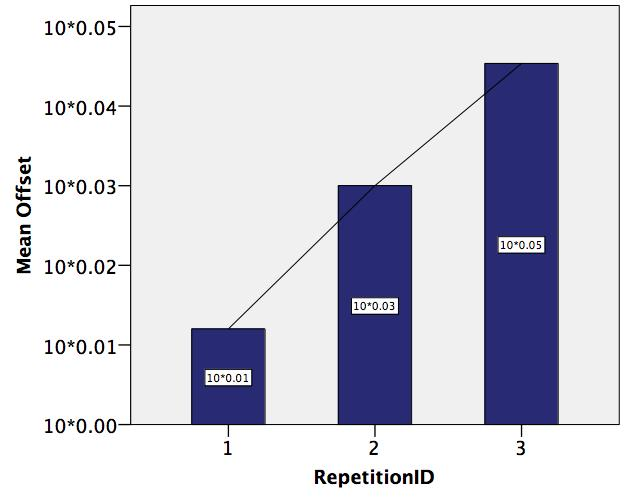
\includegraphics[width=\textwidth]{figures/learningCurveOffsetNF}
%     \caption{Error Rate Learning Curve - No Feedback Trials}
%     \label{fig:learningCurveOffsetNF}
% \end{subfigure}
% \caption{Error Rate Learning Curve}
% \label{fig:learningCurveOffset}
% \end{figure}


\begin{figure}[H]
\centering
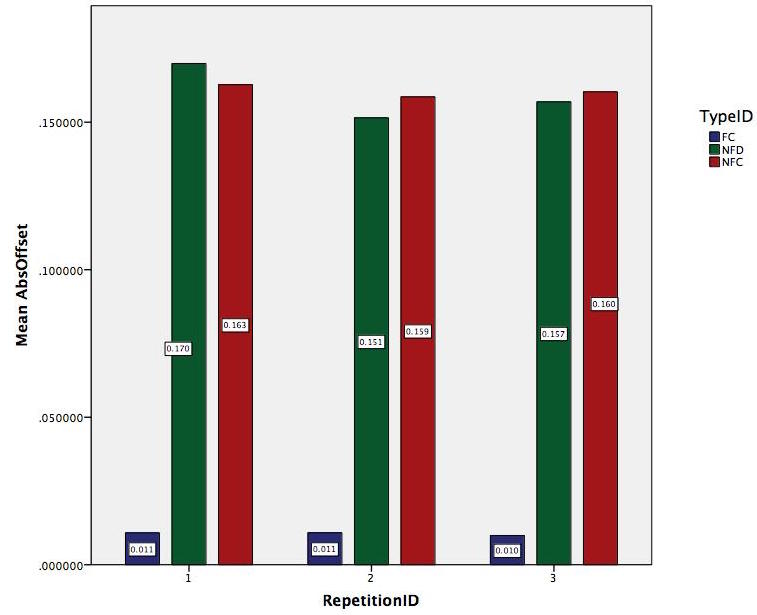
\includegraphics[width=\textwidth]{figures/learningCurveOffset}
\caption{Learning Curve - Offset}
\label{fig:learningCurveOffset}
\end{figure}


One important thing to note is, that certain values for error are affordable in No Feedback trials. Especially for No Feedback \& Discrete Targeting that maximum affordable error is presented on Table \ref{tab:NFDAffordableError}. It can be calculated using the type:

 $AffrodableError = (\frac{100}{N} = BucketSize) * \frac{1}{2}$

Affordable error is half of the size of its bucket for a specific N. Now, by combining the data from Table \ref{tab:NFDAffordableError} and Figure \ref{fig:learningCurveOffset} we can extract even more meaningful and interesting results. With the given error rates for NFD, we find that for $N=2$ or $N=3$, we will always perform selection inside the target area. That happens because the average error rates are lower than the affordable error, meaning that this error is indeed acceptable and thus we successfully performed an in-target selection. We also realize than hitting smaller targets ($N>4$), is not trivial in No Feedback trials since average error rates are much higher compared to the maximum affordable error rates for those N values.

% However, no matter of which the affordable error might have been, we still experienced quite high error rates, which were increased in each repetition. This can be partly interpreted if we take into account that No Feedback trials were really difficult for the users and required utter focusing from their side. Concentrating on the trial, was getting more and more difficult over time, due to the mental and physical fatigue. Thus users tent to have better scores on the first repetition than in the following two. In particular average error was \emph{12\%} for repetition \emph{1}, \emph{30\%} on the \emph{2nd} repetition and \emph{45\%} on the last one. This sudden and steep increase of the error values, supports our argument that users after a certain amount of time experienced fatigue and partly lost their focus on these type of trials.


\begin{table}[H]
\centering
\begin{tabular}{l || c}
N & Maximum affordable error in \% \\
\hline \hline
\textbf{2} & 25,00\% \\
\textbf{3} & 16,66\% \\
\textbf{4} & 12,50\% \\
\textbf{6} & 08,33\% \\
\textbf{8} & 06,25\% \\
\textbf{12} & 04,16\% \\
\textbf{16} & 03,12\% 
\end{tabular}
\caption{Fat Finger - No Feedback \& Discrete Targeting affordable error}
\label{tab:NFDAffordableError}
\end{table}






%%%%%%%%%%%%%%%%%%%%%%%%%%%%%
%%%%%%%%%%%%%%%%%%%%%%%%%%%%%
%%%%%%%%%%%%%%%%%%%%%%%%%%%%%
%%%%%%%%%%%%%%%%%%%%%%%%%%%%%
%%%%%%%%%%%%%%%%%%%%%%%%%%%%%
%%%%%%%%%%%%%%%%%%%%%%%%%%%%%
\section{Re-Entries}
\label{resultsReEntries}

Analysis of the target Re-Entries that occurred during the whole experiment will help us to better understand where users faced difficulties, caused by tremolo or general stabilization parameters. We meet higher values for target re-entries, when the target's range is smaller. As we will see onwards, when the finger of participant was not completely accurate and stable, the tremolo produced was enough, to cause small and usually fast movement of the feedback region. If the feedback edge was close enough to the edge of the target, then this slight movement ("in" and "out" of the target region) was encountered as 1 re-entry. 

Figure \ref{fig:meanReentries} presents the average target re-entries for each of the trial categories and  all possible \textbf{N}'s. \textbf{Feedback \& Discrete} has almost zero re-entries per trial especially for low values of N. When N increases re-entries follow along and we reach a maximum of around \emph{1.5} target re-entries per trial (\emph{N=16}). This enhances and further supports the claim we made before about the connection between target size and target re-entries.
\textbf{Feedback \& Continuous} have almost the same number of target re-entries as the size of the target is independent of the value of \emph{N}. The range of the target is even smaller that the FD one of \emph{N=16}, so the target re-entries per trial are even higher than the maximum value for Feedback \& Discrete targeting. We have an average of around 2 target re-entries for all Feedback \& Continuous trials. 
\textbf{No Feedback \& Discrete} and \textbf{No Feedback \& Continuous} have almost the same reaction regarding target re-entries. Since users are not aware of the position of the feedback region, and they need to stay inside the target for a specific time; they just move their finger in the desired position and then simply lift it. Thus, movements such as trembling around a specific area for a long time to stay accurate did not encountered. As a result target re-entries are too low; \emph{0.5} per trial or differently expressed, one every two trials. So for NF trials, target re-entries are independent both from the target's size and from the of trial (NFD or NFC). 


\begin{figure}[H]
\centering
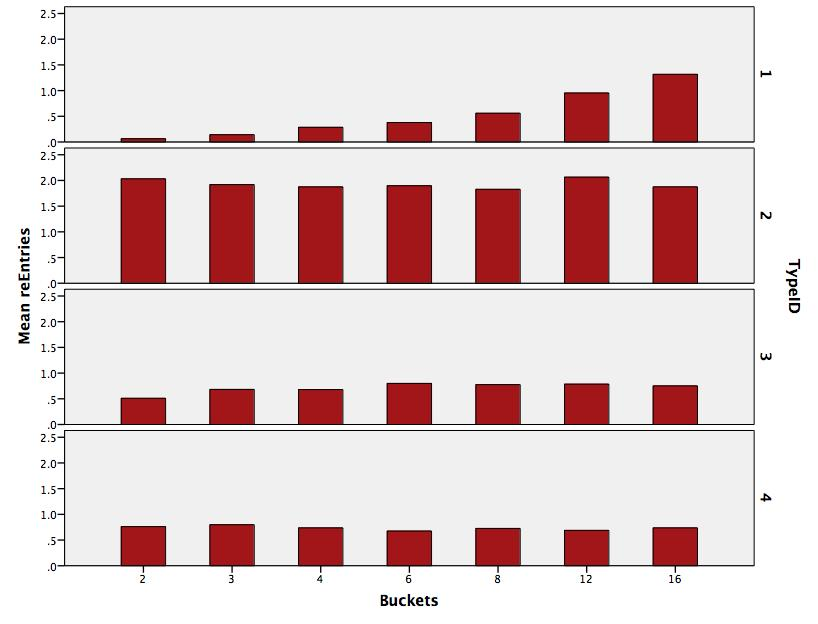
\includegraphics[scale=0.4]{figures/meanReentries}
\caption{Target Re-Entries panelled by Type of Trial}
\label{fig:meanReentries}
\end{figure}


%%%%%%%%%%%%%%%%%%%%%%%%%%%%%
%%%%%%%%%%%%%%%%%%%%%%%%%%%%%
%%%%%%%%%%%%%%%%%%%%%%%%%%%%%
%%%%%%%%%%%%%%%%%%%%%%%%%%%%%
%%%%%%%%%%%%%%%%%%%%%%%%%%%%%
%%%%%%%%%%%%%%%%%%%%%%%%%%%%%
\section{Re-Touches}
\label{resultsReTouches}

Re-touches is a parameter which is meaningful only for Feedback trials. It measures the times users re-positioned their finger by lifting it during one trial. Re-touches are not measured for No Feedback trials,  because in these trials lifting is the way to perform target selection. So, users are not allowed to reposition their finger by lifting it from the screen, because that way they will falsely select the target.
As Figure \ref{fig:meanRetouches} illustrates, Feedback \& Discrete retouches are really low, with an average of around \emph{0.6} per trial. However, for Feedback \& Continuous targeting we have a completely different pattern. Re-touches are a lot higher (around \emph{2.0} per trial) with small diversities for \emph{N=2} and \emph{N=12}. However, I point out two significant observations that were extracted from the comments section of the assessment participants filled in after the experiment.

\begin{enumerate}
     \item Users had many difficulties to hit continuous targets that were really close to the minimum point. Because the red line is randomly positioned within each bucket, in case it is really close to the minimum point, selection of the target becomes a cumbersome task. They usually had to perform several re-touches and re-entries to be able to select the target.  

     \item The above behaviour was also encountered when the target was close to the maximum area but not exactly on it. Then participants faced the same difficulties, to avoid tremolo and stabilize their finger. 
 \end{enumerate} 

 We conclude that for targets placed really close to the minimum or the maximum calibrated ones, the ability to control the feedback line is significantly decreased. This is probably not happening due to software reasons, but possible because of other ergonomic issues of the finger. 

\begin{figure}[h]
\centering
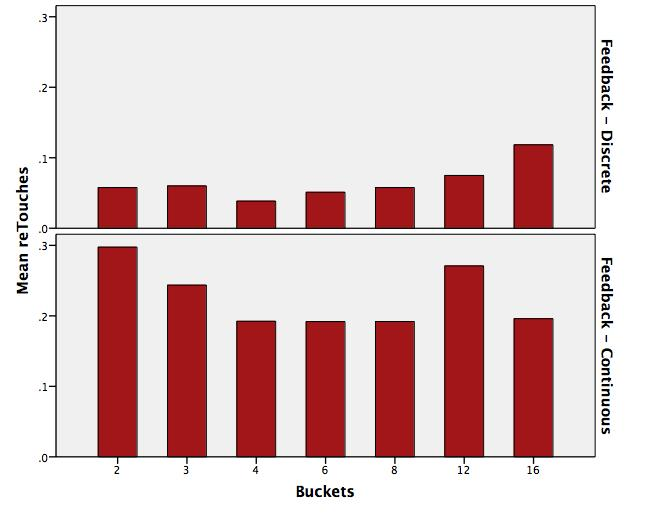
\includegraphics[scale=0.4]{figures/meanRetouches}
\caption{Target Re-Touches for Feedback Trials}
\label{fig:meanRetouches}
\end{figure}



%%%%%%%%%%%%%%%%%%%%%%%%%%%%%
%%%%%%%%%%%%%%%%%%%%%%%%%%%%%
%%%%%%%%%%%%%%%%%%%%%%%%%%%%%
%%%%%%%%%%%%%%%%%%%%%%%%%%%%%
%%%%%%%%%%%%%%%%%%%%%%%%%%%%%
%%%%%%%%%%%%%%%%%%%%%%%%%%%%%
\section{Subjective Preferences}
\label{resultsSubjectivePreferences}

In Figure \ref{fig:meanQuestGraphs}, the mean values for all the parts of the assessment presented in section \ref{assessment} are illustrated and presented. On each diagram the vertical axis represents the mean values of the corresponding category, which are ranged from 1 to 5 (5 point Likert scale). Generally, higher values mean that participants positively rated the specified category. The horizontal axis corresponds to the type of Trial. Each graph has 4 columns, identified with the numbers 1-4, which correspond to the respective type of trials.

\begin{figure}[h]
    \centering
    \begin{subfigure}[b]{0.4\textwidth}
        \centering
        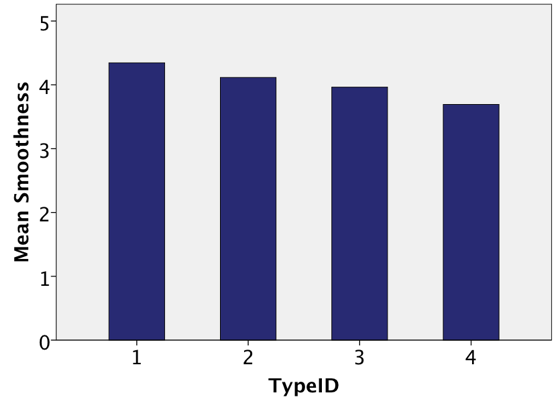
\includegraphics[width=\textwidth]{figures/meanSmoothness}
        \caption{Mean Smoothness}
        \label{fig:meanSmoothness}
    \end{subfigure}
    \hfill
    \begin{subfigure}[b]{0.4\textwidth}
        \centering
        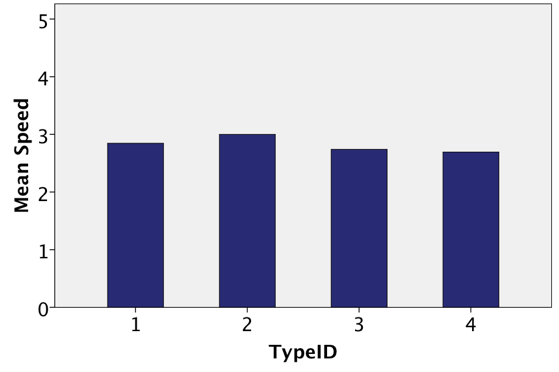
\includegraphics[width=\textwidth]{figures/meanSpeed}
        \caption{Mean Speed }
        \label{fig:meanSpeed}
    \end{subfigure}
    \hfill
    \begin{subfigure}[b]{0.4\textwidth}
        \centering
        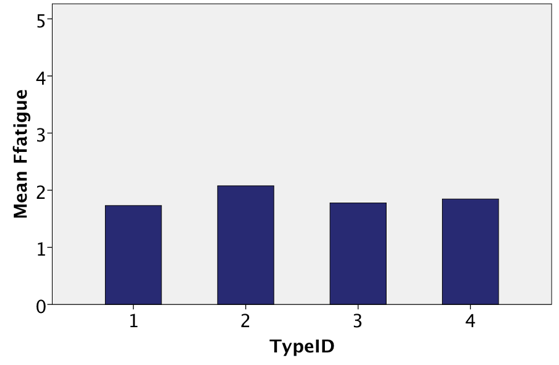
\includegraphics[width=\textwidth]{figures/meanFFatigue}
        \caption{Mean finger Fatigue}
        \label{fig:meanFFatigue}
    \end{subfigure}
    \hfill
    \begin{subfigure}[b]{0.4\textwidth}
        \centering
        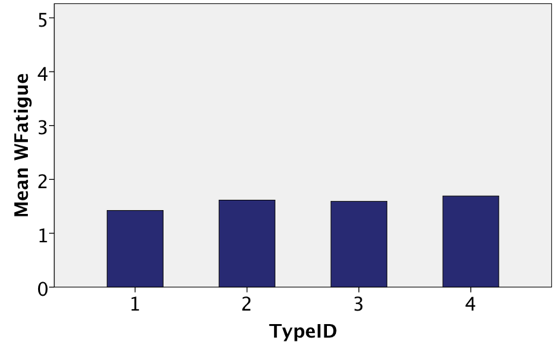
\includegraphics[width=\textwidth]{figures/meanWFatigue}
        \caption{Mean Wrist Fatigue}
        \label{fig:meanWFatigue}
    \end{subfigure}
    \hfill
    \begin{subfigure}[b]{0.4\textwidth}
        \centering
        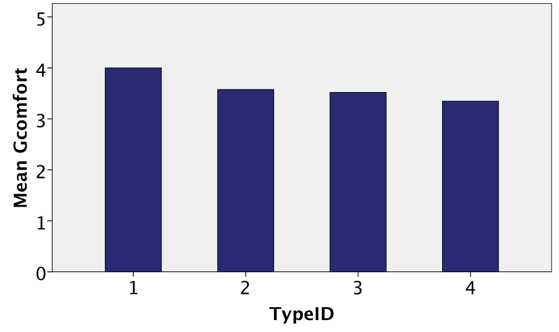
\includegraphics[width=\textwidth]{figures/meanGComfort}
        \caption{Mean Smoothness during operation}
        \label{fig:meanGComfort}
    \end{subfigure}
    \hfill
    \begin{subfigure}[b]{0.4\textwidth}
        \centering
        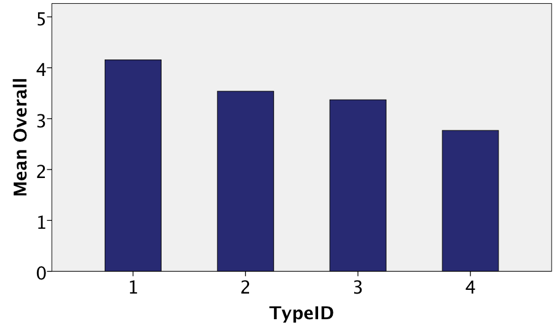
\includegraphics[width=\textwidth]{figures/meanOverall}
        \caption{Mean Overall Performance}
        \label{fig:meanOverall}
    \end{subfigure}
    \caption{Mean Values assessed by participants for each trial category}
    \label{fig:meanQuestGraphs}
\end{figure}

FD(1) scored consistently well across all the above categories. It scored mean values that were always improved than the ones of other trials. 
Precisely, Feedback \& Discrete Targeting (1) was ranked higher concerning the Overall Performance (\emph{mean = 3.46 / 5}), Figure \ref{fig:meanOverall}. It can be observed that overall performance is decreased as the identification of the type of trial is increasing. The same behavior is also noticed for Mean Smoothness (\emph{mean = 4.03 / 5}), Figure \ref{fig:meanSmoothness}. However Most importantly, all four techniques ranked amazingly concerning the Fatigue of both the finger and the wrist. Even being an extensive and long experiment, which might not well correspond to everyday use scenario,  the fatigue  participants experienced was in extremely low levels. Finger fatigue had \emph{mean = 1.86}, as shown in Figure \ref{fig:meanFFatigue}, and Wrist fatigue also had \emph{mean = 1.58}, as shown in Figure \ref{fig:meanWFatigue}. Concerning Speed (\emph{mean = 2.82}), Figure \ref{fig:meanSpeed}, all techniques ranged quite uniformly, outlining that the operational speed of the experiment and of each technique in particular was mostly normal. Finally, Smoothness (\emph{mean = 4.03 / 5}), Figure \ref{fig:meanOverall}, ranged also very high for all techniques, which proves that our application is well structured and well corresponds to the movement of the finger.




% \begin{figure}[h]
% \centering
% 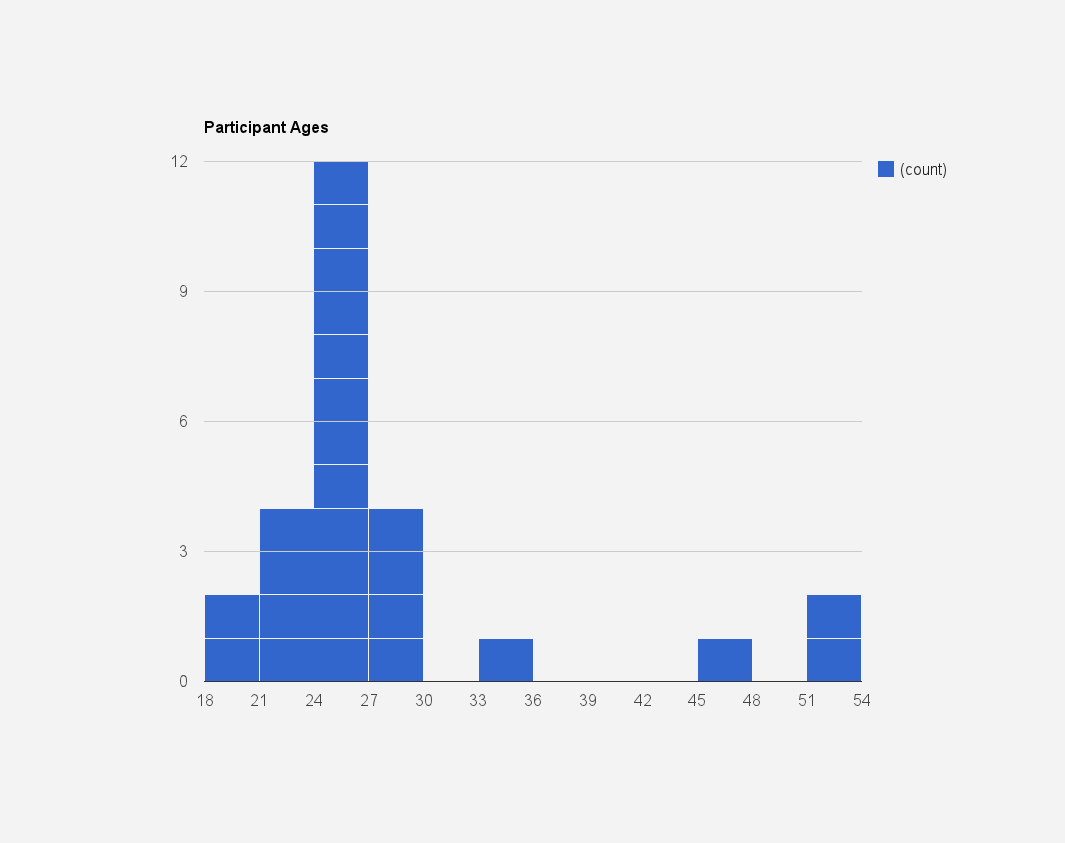
\includegraphics[scale=0.5]{figures/participantAge.png}
% \caption{Distribution of participant ages}
% \label{fig:participantAge}
% \end{figure}



% \begin{itemize}
% \item \textbf{}
% \item \textbf{}
% \item \textbf{}
% \item \textbf{}
% \end{itemize}